% Options for packages loaded elsewhere
\PassOptionsToPackage{unicode}{hyperref}
\PassOptionsToPackage{hyphens}{url}
%
\documentclass[
]{article}
\usepackage{amsmath,amssymb}
\usepackage{lmodern}
\usepackage{iftex}
\ifPDFTeX
  \usepackage[T1]{fontenc}
  \usepackage[utf8]{inputenc}
  \usepackage{textcomp} % provide euro and other symbols
\else % if luatex or xetex
  \usepackage{unicode-math}
  \defaultfontfeatures{Scale=MatchLowercase}
  \defaultfontfeatures[\rmfamily]{Ligatures=TeX,Scale=1}
\fi
% Use upquote if available, for straight quotes in verbatim environments
\IfFileExists{upquote.sty}{\usepackage{upquote}}{}
\IfFileExists{microtype.sty}{% use microtype if available
  \usepackage[]{microtype}
  \UseMicrotypeSet[protrusion]{basicmath} % disable protrusion for tt fonts
}{}
\makeatletter
\@ifundefined{KOMAClassName}{% if non-KOMA class
  \IfFileExists{parskip.sty}{%
    \usepackage{parskip}
  }{% else
    \setlength{\parindent}{0pt}
    \setlength{\parskip}{6pt plus 2pt minus 1pt}}
}{% if KOMA class
  \KOMAoptions{parskip=half}}
\makeatother
\usepackage{xcolor}
\IfFileExists{xurl.sty}{\usepackage{xurl}}{} % add URL line breaks if available
\IfFileExists{bookmark.sty}{\usepackage{bookmark}}{\usepackage{hyperref}}
\hypersetup{
  hidelinks,
  pdfcreator={LaTeX via pandoc}}
\urlstyle{same} % disable monospaced font for URLs
\usepackage[margin=1in]{geometry}
\usepackage{color}
\usepackage{fancyvrb}
\newcommand{\VerbBar}{|}
\newcommand{\VERB}{\Verb[commandchars=\\\{\}]}
\DefineVerbatimEnvironment{Highlighting}{Verbatim}{commandchars=\\\{\}}
% Add ',fontsize=\small' for more characters per line
\usepackage{framed}
\definecolor{shadecolor}{RGB}{248,248,248}
\newenvironment{Shaded}{\begin{snugshade}}{\end{snugshade}}
\newcommand{\AlertTok}[1]{\textcolor[rgb]{0.94,0.16,0.16}{#1}}
\newcommand{\AnnotationTok}[1]{\textcolor[rgb]{0.56,0.35,0.01}{\textbf{\textit{#1}}}}
\newcommand{\AttributeTok}[1]{\textcolor[rgb]{0.77,0.63,0.00}{#1}}
\newcommand{\BaseNTok}[1]{\textcolor[rgb]{0.00,0.00,0.81}{#1}}
\newcommand{\BuiltInTok}[1]{#1}
\newcommand{\CharTok}[1]{\textcolor[rgb]{0.31,0.60,0.02}{#1}}
\newcommand{\CommentTok}[1]{\textcolor[rgb]{0.56,0.35,0.01}{\textit{#1}}}
\newcommand{\CommentVarTok}[1]{\textcolor[rgb]{0.56,0.35,0.01}{\textbf{\textit{#1}}}}
\newcommand{\ConstantTok}[1]{\textcolor[rgb]{0.00,0.00,0.00}{#1}}
\newcommand{\ControlFlowTok}[1]{\textcolor[rgb]{0.13,0.29,0.53}{\textbf{#1}}}
\newcommand{\DataTypeTok}[1]{\textcolor[rgb]{0.13,0.29,0.53}{#1}}
\newcommand{\DecValTok}[1]{\textcolor[rgb]{0.00,0.00,0.81}{#1}}
\newcommand{\DocumentationTok}[1]{\textcolor[rgb]{0.56,0.35,0.01}{\textbf{\textit{#1}}}}
\newcommand{\ErrorTok}[1]{\textcolor[rgb]{0.64,0.00,0.00}{\textbf{#1}}}
\newcommand{\ExtensionTok}[1]{#1}
\newcommand{\FloatTok}[1]{\textcolor[rgb]{0.00,0.00,0.81}{#1}}
\newcommand{\FunctionTok}[1]{\textcolor[rgb]{0.00,0.00,0.00}{#1}}
\newcommand{\ImportTok}[1]{#1}
\newcommand{\InformationTok}[1]{\textcolor[rgb]{0.56,0.35,0.01}{\textbf{\textit{#1}}}}
\newcommand{\KeywordTok}[1]{\textcolor[rgb]{0.13,0.29,0.53}{\textbf{#1}}}
\newcommand{\NormalTok}[1]{#1}
\newcommand{\OperatorTok}[1]{\textcolor[rgb]{0.81,0.36,0.00}{\textbf{#1}}}
\newcommand{\OtherTok}[1]{\textcolor[rgb]{0.56,0.35,0.01}{#1}}
\newcommand{\PreprocessorTok}[1]{\textcolor[rgb]{0.56,0.35,0.01}{\textit{#1}}}
\newcommand{\RegionMarkerTok}[1]{#1}
\newcommand{\SpecialCharTok}[1]{\textcolor[rgb]{0.00,0.00,0.00}{#1}}
\newcommand{\SpecialStringTok}[1]{\textcolor[rgb]{0.31,0.60,0.02}{#1}}
\newcommand{\StringTok}[1]{\textcolor[rgb]{0.31,0.60,0.02}{#1}}
\newcommand{\VariableTok}[1]{\textcolor[rgb]{0.00,0.00,0.00}{#1}}
\newcommand{\VerbatimStringTok}[1]{\textcolor[rgb]{0.31,0.60,0.02}{#1}}
\newcommand{\WarningTok}[1]{\textcolor[rgb]{0.56,0.35,0.01}{\textbf{\textit{#1}}}}
\usepackage{graphicx}
\makeatletter
\def\maxwidth{\ifdim\Gin@nat@width>\linewidth\linewidth\else\Gin@nat@width\fi}
\def\maxheight{\ifdim\Gin@nat@height>\textheight\textheight\else\Gin@nat@height\fi}
\makeatother
% Scale images if necessary, so that they will not overflow the page
% margins by default, and it is still possible to overwrite the defaults
% using explicit options in \includegraphics[width, height, ...]{}
\setkeys{Gin}{width=\maxwidth,height=\maxheight,keepaspectratio}
% Set default figure placement to htbp
\makeatletter
\def\fps@figure{htbp}
\makeatother
\setlength{\emergencystretch}{3em} % prevent overfull lines
\providecommand{\tightlist}{%
  \setlength{\itemsep}{0pt}\setlength{\parskip}{0pt}}
\setcounter{secnumdepth}{-\maxdimen} % remove section numbering
\ifLuaTeX
  \usepackage{selnolig}  % disable illegal ligatures
\fi

\author{}
\date{\vspace{-2.5em}}

\begin{document}

\hypertarget{assignment-1-r-markdown-practice}{%
\section{Assignment 1: R Markdown
practice}\label{assignment-1-r-markdown-practice}}

\begin{quote}
\hypertarget{important}{%
\subsubsection{Important}\label{important}}

Before you start working on this assignment you first need to set-up
RStudio. If you have already worked through the first CDS 102 lab (Lab
0), then you do not need to do this again. Otherwise, please follow all
the directions in this section of the supplementary textbook:
\href{https://book.cds101.com/initial-set-up.html}{RStudio Initial
Set-up}
\end{quote}

\hypertarget{overview}{%
\subsection{Overview}\label{overview}}

The goal of this assignment is to recreate
\href{https://gmuedu-my.sharepoint.com/:b:/g/personal/dwhite34_gmu_edu/ESKWurLFXaFKnqnAo-krkXEBPP6h7gz9Fe-JIVPJCjzEhg?e=92BgLP}{this
example PDF file}.

\hypertarget{instructions}{%
\subsection{Instructions}\label{instructions}}

\begin{enumerate}
\def\labelenumi{\arabic{enumi}.}
\item
  Follow the instructions on Blackboard and
  \href{https://book.cds101.com/using-rstudio-server-to-clone-a-github-repo-as-a-new-project.html}{here}
  to open this repository in RStudio Server as a new project.
\item
  In the bottom right pane of RStudio is a \emph{Files} tab. Once you
  have opened this assignment as a Project in RStudio, you will see a
  list of files here. Click on the file called
  \texttt{rmarkdown\_practice.Rmd}. The file should open in a new editor
  pane in the top right of RStudio.
\item
  Take a look at the contents of the RMarkdown file. It should look
  something like this:

  \begin{figure}
  \centering
  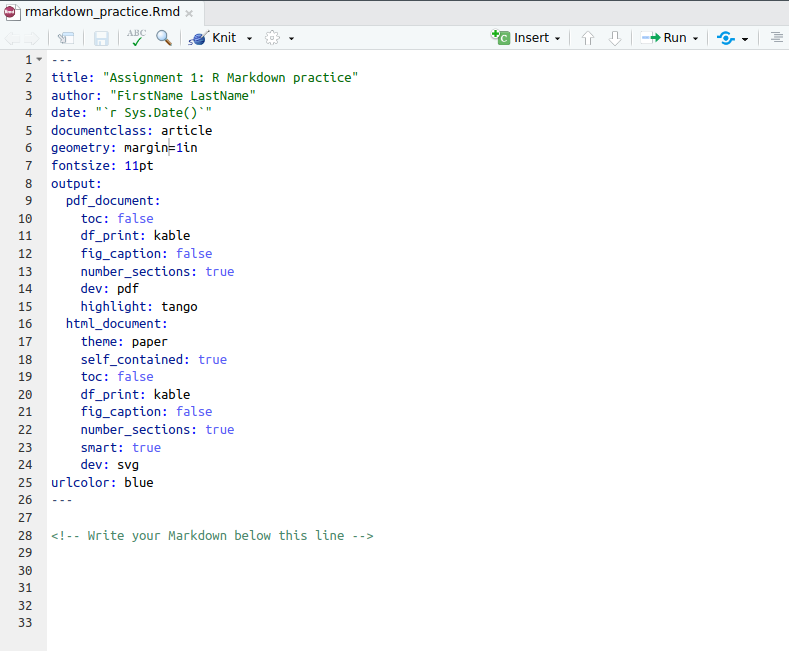
\includegraphics{img/rmd-starter-file.png}
  \caption{Initial contents of RMarkdown file}
  \end{figure}

  To convert the RMarkdown file into an output PDF file, click the
  \emph{Knit} button at the top of the editing pane. You should see a
  PDF appear, corresponding to the current contents of the
  \texttt{rmarkdown\_practice.Rmd} file.

  \begin{quote}
  Depending on your operating system/browser you may have to allow
  pop-ups, or click the PDF file that has appeared in the PDF pane.
  \end{quote}
\item
  Your goal for this assignment is to edit the contents of the
  \texttt{rmarkdown\_practice.Rmd} file in RStudio so that when you Knit
  it to a PDF, it matches the contents and formatting of this example
  file (except for the diagonal watermark, the name, and the date):
  \href{https://gmuedu-my.sharepoint.com/:b:/g/personal/dwhite34_gmu_edu/ESKWurLFXaFKnqnAo-krkXEBPP6h7gz9Fe-JIVPJCjzEhg?e=92BgLP}{\texttt{rmarkdown\_example.pdf}}.

  Let's start by fixing the name. This is inserted into the PDF based on
  the author specified in the header section of the Rmd file (the header
  section contains formatting instructions, and is between the
  \texttt{-\/-\/-} on lines 1-26).

  Find the \texttt{author} line in the header section, and replace
  \texttt{FirstName\ LastName} with your first and last name. Keep the
  quotation marks.

  As soon as you edit the file, you will notice that the name of the
  file at the top editor tab for this \texttt{rmarkdown\_practice.Rmd}
  has changed color: it should now be red with an asterisk after it:

  \begin{figure}
  \centering
  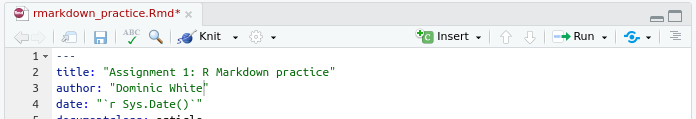
\includegraphics{img/rmd-unsaved.png}
  \caption{Initial contents of RMarkdown file}
  \end{figure}

  This indicates that the file is unsaved. Click the save icon at the
  top of the editor pane (or press Ctrl+S {[}Cmd+S on a Mac{]}). The
  file name should become black, indicating your work has been saved.

  Now Knit the file again. You should see that the resulting PDF has
  been updated to contain your name.
\item
  As well as saving the file normally, we will also be using Git to
  create checkpoints in the history of our project as we work on it. The
  checkpoints allow us to easily track the history of edits in the
  project (much like ``Track Changes'' in a Word document). We can also
  share this history of checkpoints (and work collaboratively) by
  uploading our checkpoints \& edits to a shared website like GitHub.

  Some useful terminology:

  \begin{itemize}
  \tightlist
  \item
    \textbf{Commit}: the name for the checkpoints that we make
  \item
    \textbf{Staging}: staging a file means that you want to include any
    edits to it in the next commit.
  \item
    \textbf{Pushing}: the process of uploading your work to GitHub.
  \end{itemize}

  When you first created the repository, there was a table of files near
  the top of the page. At the top of this table was a highlighted blue
  line that looked like this:

  \begin{figure}
  \centering
  
\includegraphics{img/github-commit-info.png}
  \caption{GitHub commit information}
  \end{figure}

  If you look on the homepage for your repository on GitHub you should
  see something similar (The URL of this respository will be something
  like:
  \texttt{https://github.com/mason-sp21-cds101/assignment-1-yourGithubUsername}).
  This line tells you about the most recent commit (checkpoint) that was
  pushed (uploaded) to GitHub for this project. Right now there is just
  one commit, which is attributed to one of the CDS 101 professors.

  Let's add the change you just made to the project history! Follow
  \href{https://book.cds101.com/how-to-stage-commit-and-push-to-github-using-rstudio-server.html}{these
  instructions in the supplementary textbook} to stage, commit, and push
  your work in the \texttt{rmarkdown\_practice.Rmd} file to GitHub.
  (When you get to the commit message in Step 3, type something
  descriptive about the work you did, such as \emph{Changed author
  name}.)

  Once you have successfully pushed your work, go back to the web page
  for your the GitHub repository for Assignment 1. Refresh the page.

  \begin{itemize}
  \tightlist
  \item
    You should see that the blue header of information has updated - it
    should now say that there are two commits, and show that the most
    recent one was just created by you, along with the commit message
    that you created and the time of the commit!
  \item
    If you look down the list of files below the blue header, you can
    also see that GitHub shows you the last commit that modified that
    file.
  \end{itemize}

  \begin{quote}
  If you do not see this line change, you may need to ``force'' refresh
  the webpage:
  \href{https://www.wikihow.com/Force-Refresh-in-Your-Internet-Browser}{instructions
  for different OS/browsers}.

  If that still doesn't work, make sure that you committed and pushed
  the \texttt{rmarkdown\_practice.Rmd} file correctly, without any error
  messages.
  \end{quote}
\item
  Let's get back to reproducing the
  \href{https://gmuedu-my.sharepoint.com/:b:/g/personal/dwhite34_gmu_edu/ESKWurLFXaFKnqnAo-krkXEBPP6h7gz9Fe-JIVPJCjzEhg?e=92BgLP}{example
  file} in RStudio. However, keep in mind that it's a good idea to
  commit your work frequently. You can push after each commit or after
  several commits, but bear in mind that pushing to GitHub is a good way
  of backing up your work.

  The date in the output PDF is automatically set to the current date by
  date line in the RMarkdown header (line 4), so we do not need to
  change that. Let's move onto the content of the file.

  Scroll down to line 30 of the \texttt{rmarkdown\_practice.Rmd} file
  and type a word or two, e.g.~\emph{Hello World!}.

  Then Knit to PDF again - you should see that the text you just added
  appears in the PDF.
\item
  We can use special symbols to control how this text is formatted. For
  example, to convert this line to a heading, put \texttt{\#} at the
  start of the line. I.e. replace \texttt{Hello\ World!} on line 8 with
  \texttt{\#\ Hello\ World}.

  Knit again - you should see that the \texttt{\#} is not in the PDF,
  but the line has been converted into a large heading, and
  automatically numbered for us.

  Try replacing \texttt{\#} with \texttt{\#\#} in the RMarkdown file -
  what happens?

  Now go back to the example PDF that we are trying to reproduce, and
  fill in the correct heading.

  Keep editing and knitting the PDF until you've got that first heading
  correct. Then commit and push the \texttt{rmarkdown\_practice.Rmd}
  file to GitHub. (Use a short but descriptive commit message for the
  work that you did, such as \emph{Added first heading}). You should now
  see that you have 3 commits in your GitHub repository!
\item
  A guide to all the different formatting symbols you can use in an
  RMarkdown document is given in this PDF:
  \href{https://www.rstudio.com/wp-content/uploads/2015/03/rmarkdown-reference.pdf}{\texttt{RMarkdown\ reference\ guide}}

  Enter the text you see in the example PDF into the
  \texttt{rmarkdown\_practice.Rmd} file, and then find the formatting
  symbols you need to match the formatting to the example PDF.

  Other instructions:

  \begin{itemize}
  \item
    Make sure to replace the section with the actual section that you
    are in. If you are unsure what this is, look it up in the syllabus,
    on Blackboard, or in PatriotWeb.
  \item
    The second section of the PDF contains a bullet point list. Note
    that (1) there is a second nested list under the first bullet point
    of this list, and (2) the blue word GitHub is a link to a webpage.
    You will need to look up the formatting symbols to reproduce all of
    these.
  \item
    The final part of the document contains two \emph{R code chunks}.
    These runs the code in the chunk and automatically inserts the
    output of the code below the chunk when you knit the file. Look up
    the opening and closing formatting symbols for a code chunk in the
    \href{https://www.rstudio.com/wp-content/uploads/2015/03/rmarkdown-reference.pdf}{\texttt{RMarkdown\ reference\ guide}}
    PDF.
  \item
    Make sure you put blank lines between different
    paragraphs/headings/lists/etc. Text on consecutive lines will be
    treated as the same line when RStudio knits your file. For example:

\begin{Shaded}
\begin{Highlighting}[]
\NormalTok{Some regular text.}
\FunctionTok{\# An Important Heading}
\end{Highlighting}
\end{Shaded}

    would be knitted to:

    Some regular text.\# An Important Heading

    which is probably not what you intended\ldots{}
  \item
    Make sure you don't have spaces at the start of lines unless you
    intended to. Spaces at the start of lines are actually formatting
    symbols, so this can make your output look different to what you
    intended. For example, spaces before a bullet point will created a
    nested list within a list.
  \item
    Commit at frequent intervals - we want to see at least 5 or 6
    commits on GitHub by the time you are finished with the assignment.
  \end{itemize}
\end{enumerate}

When you're finished, follow the directions in the
\textbf{\protect\hyperlink{how-to-submit}{How to submit}} section below.

\hypertarget{how-to-submit}{%
\subsection{How to submit}\label{how-to-submit}}

To submit your assignment, follow the two steps below. Your assignment
will be graded for credit \textbf{after} you've completed both steps!

\begin{enumerate}
\def\labelenumi{\arabic{enumi}.}
\item
  Save, commit, and push your completed R Markdown file so that
  everything is synchronized to GitHub. If you do this right, then you
  will be able to view your completed file on the GitHub website.
\item
  Knit your R Markdown document to the PDF format, export (download) the
  PDF file from RStudio Server, and then upload it to the
  \emph{Assignment 1} posting on Blackboard.
\end{enumerate}

\hypertarget{cheatsheets}{%
\subsection{Cheatsheets}\label{cheatsheets}}

You should keep the following reference handy while working on this
assignment:

\begin{itemize}
\tightlist
\item
  \href{https://www.rstudio.com/wp-content/uploads/2015/03/rmarkdown-reference.pdf}{RMarkdown
  reference}
\end{itemize}

\end{document}
